%*****************************************
\chapter{Multiple Sheets}\label{ch06:multiple_sheets}
%*****************************************

Excel workbooks often contain a large amount of data and worksheets can quickly become overwhelming. When one worksheet becomes cumbersome, data can be broken out into smaller subsets and placed in separate worksheets within the same Excel file. Separating out spreadsheet data into smaller pieces can lead to better data organization within a file and increase its ease of use. When a retail company needs to track overall sales along with individual store sales, it makes sense to place each store's sales data in a separate sheet within a file. Adding a summary sheet that sums across all the sheets will total the entire company sales data in the same file. This chapter will show how to set up a workbook to make multi-sheet formulas quick and easy.

Other examples of when multiple sheets make the most sense are when comparing regional data for a company, data for a sales force where individual salesperson performance is analyzed along with overall sales, and data over a period of time where sheets can be broken out by year or by month. When comparing data across several sheets, it is essential that all the sheets are laid out in the same way. To facilitate this, a template can be used. A template is the basic pattern for each new sheet that can be used repeatedly to make sure each new sheet has the same setup, formatting, formulas, etc. as the existing sheets in a file. In this chapter, both predefined Excel templates and those created from scratch will be used to meet the specific needs of the work required.

\section{Multiple Sheet Basics}

\begin{center}
	\begin{objbox}{Learning Objectives}
		\begin{itemize}
			\setlength{\itemsep}{0pt}
			\setlength{\parskip}{0pt}
			\setlength{\parsep}{0pt}
			
			\item Navigating through a multiple sheet file.
			\item Adding, deleting, copying, and moving sheets.
			\item Grouping and ungrouping sheets.

		\end{itemize}
	\end{objbox}
\end{center}

The Excel workbooks used throughout this textbook have included multiple sheets. This chapter develops a personal budget file that contains income and expenses for an entire year. The file contains a sheet for each month of the year as well as a Summary sheet that totals all twelve monthly sheets of data together. The chapter begins with exercises designed to demonstrate moving through worksheets, organizing them, and making sure that all twelve monthly sheets are consistent. Figure \ref{06:fig01} shows the \fmtWorksheetName{January} sheet in the \fmtWorkbookName{Personal Budget} file along with all the sheet tabs along the bottom of the window.

\begin{figure}[H]
	\centering
	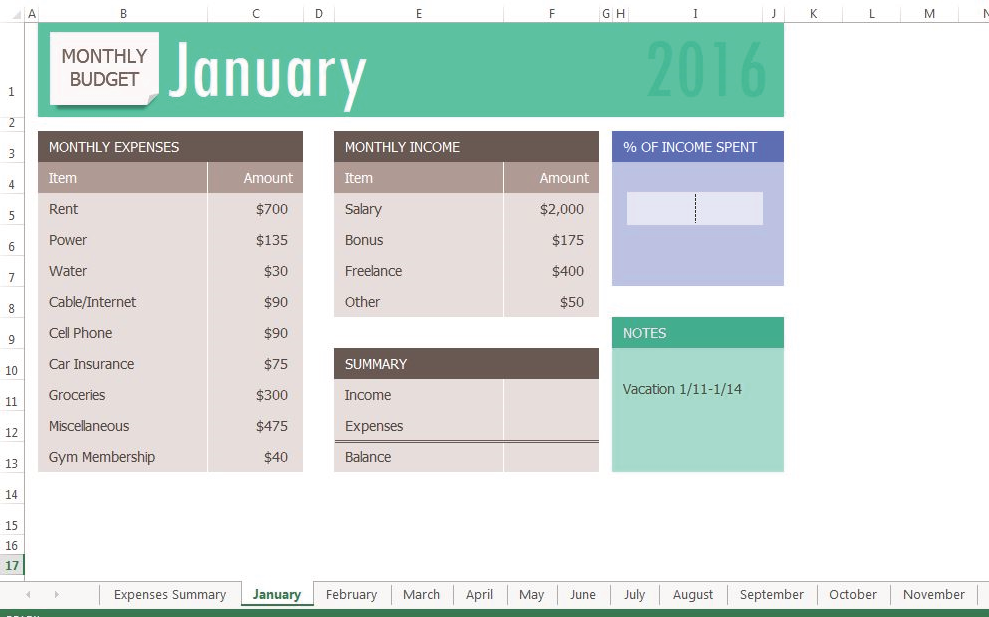
\includegraphics[width=\maxwidth{.95\linewidth}]{gfx/ch06_fig01}
	\caption{January Sheet in the Personal Budget File}
	\label{06:fig01}
\end{figure}

\subsection{Navigating Through a Multiple Sheet File}

\textit{Data file: CH6 Data}

\begin{enumerate}
	\item Open the data file \fmtWorkbookName{CH6 Data} and save the file as \fmtWorkbookName{CH6 Personal Budget}. Notice that the file has an \fmtWorksheetName{Expenses Summary} sheet tab at the far left followed by monthly sheets.
	\item Click on the different sheet tabs at the bottom of the screen to move through the sheets. Notice that the \fmtWorksheetName{Expenses Summary} sheet is formatted differently from the monthly sheets. Notice also that all the monthly sheets are identical in layout and format.
	\item Take a second look at the months and notice the end of the year data for September through October has not been added and there is no sheet for December. 
	\item Add the following data in the \fmtWorksheetName{September}, \fmtWorksheetName{October}, and \fmtWorksheetName{November} sheets.
\end{enumerate}

\begin{table}[H]
	\rowcolors{1}{}{tablerow} % zebra striping background
	{\small
		%\fontsize{8}{10} \selectfont %Replace small for special font size
		\begin{longtable}{L{1.0in}L{0.75in}L{0.75in}L{0.75in}} %Left-aligned, Max width: 4.25in
			\textbf{Item} & \textbf{September} & \textbf{October} & \textbf{November} \endhead
			\hline
			Power         & $ \$135 $ & $ \$135 $ & $ \$135 $ \\
			Water         & $ \$30 $  & $ \$30 $  & $ \$30 $  \\
			Groceries     & $ \$300 $ & $ \$325 $ & $ \$400 $ \\
			Miscellaneous & $ \$100 $ & $ \$50 $  & $ \$100 $ \\
			Bonus         &           &           &           \\
			Freelance     & $ \$500 $ &           & $ \$150 $ \\
			Other         &           & $ \$100 $ &           \\

			\rowcolor{captionwhite}
			\caption{Data for September/October/November}
			\label{06:tab01}
		\end{longtable}
	}
\end{table}

\subsection{Copying a Sheet}

To make a \fmtWorksheetName{December} sheet, copy the \fmtWorksheetName{November} sheet.

\begin{enumerate}
	\item Point the mouse at the \fmtWorksheetName{November} sheet tab at the bottom of the screen.
	\item Hold down the left mouse button and then press and hold down the \fmtKeystroke{Ctrl} key.
	\item At this point, notice a black down-pointing arrow to the left of the \fmtWorksheetName{November} sheet tab and the mouse cursor becomes a small piece of paper with a plus sign on it.
	\item Drag the mouse to the right (still holding down the left-mouse button and the \fmtKeystroke{Ctrl} key) until the black down-pointing arrow is to the right of the \fmtWorksheetName{November} sheet tab.
	\item Let go of the mouse button and then the \fmtKeystroke{Ctrl} key. There should now be a \fmtWorksheetName{November (2)} sheet to the right of the \fmtWorksheetName{November} sheet as shown in Figure \ref{06:fig02}.
\end{enumerate}

\begin{figure}[H]
	\centering
	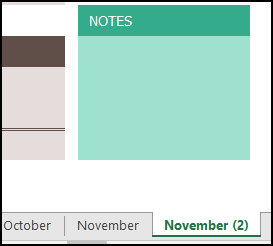
\includegraphics[width=\maxwidth{.95\linewidth}]{gfx/ch06_fig02}
	\caption{Additional November Sheet}
	\label{06:fig02}
\end{figure}

Next, update the \fmtWorksheetName{November (2)} sheet to turn it into the \fmtWorksheetName{December} sheet.

\begin{enumerate}
	\item Right-click on the \fmtWorksheetName{November (2)} sheet name at the bottom of the screen and choose \fmtPopupButton{Rename}.
	\item Type \fmtTyping{December} and press \fmtKeystroke{Enter}.
	\item Click on the \fmtWorksheetName{December} sheet.
	\item Click on \fmtCellLocation{B1} and change \textit{November} to \fmtTyping{December}.
	\item Make the following data changes.

	\begin{itemize}
		\item Miscellaneous: $ \$300 $
		\item Bonus: $ \$250 $ (holiday bonus)
		\item Freelance: delete amount
	\end{itemize}

	\item Save the workbook.
	\item Point the mouse at the \fmtWorksheetName{December} sheet tab at the bottom of the screen.
	\item Hold down the left mouse button and then press and hold down the \fmtKeystroke{Ctrl} key.
	\item Drag the mouse to the right (still holding down the left-mouse button and the \fmtKeystroke{Ctrl} key) until the black down-pointing arrow is to the right of the \fmtWorksheetName{December} sheet.
	\item Let go of the mouse button and then the \fmtKeystroke{Ctrl} key. There should now be a \fmtWorksheetName{December (2)} sheet to the right of the \fmtWorksheetName{December} sheet.
	\item Rename the \fmtWorksheetName{December(2)} sheet to \fmtTyping{Practice}.
\end{enumerate}

\begin{center}
	\begin{sklbox}{Skill Refresher}
		\textbf{Copying a Sheet}
		\\
		\begin{itemize}
			\setlength{\itemsep}{0pt}
			\setlength{\parskip}{0pt}
			\setlength{\parsep}{0pt}
			
			\item Point the mouse at the sheet to copy at the bottom of the screen.
			\item Hold down the left mouse button and then press and hold down the \fmtKeystroke{Ctrl} key.
			\item Drag the mouse to the right (still holding down the left-mouse button and the \fmtKeystroke{Ctrl} key) until the black down-pointing arrow is to the right of the existing sheet.
			\item Let go of the mouse button and then the \fmtKeystroke{Ctrl} key. There should now be a \fmtWorksheetName{Sheetname (2)} to the right of the original sheet.
			\item Rename the \fmtWorksheetName{Sheetname (2)} sheet as desired.
			
		\end{itemize}
	\end{sklbox}
\end{center}

\subsection{Moving and Deleting Sheets}

Sometimes worksheets do not end up in the right order, and they need to be moved.

\begin{enumerate}
	\item Point to the \fmtWorksheetName{Practice} sheet and hold down the left mouse button.
	\item Notice this time that there is still a black arrow to the left of the \fmtWorksheetName{Practice} sheet, but the piece of paper is blank. It does not have a plus sign ($ + $) because the sheet is moving instead of copying.
	\item Left-drag the mouse to the right until the black arrow marker is between the \fmtWorksheetName{October} and \fmtWorksheetName{November} sheets.
	\item Release the mouse button.
	\item Try moving the \fmtWorksheetName{Practice} sheet back to the right of the \fmtWorksheetName{December} sheet.
\end{enumerate}

Since the \fmtWorksheetName{Practice} sheet is not needed in the \fmtWorkbookName{Budget} file, delete it now.

\begin{enumerate}
	\item Right-click on the \fmtWorksheetName{Practice} sheet tab at the bottom of the screen.
	\item Click \fmtPopupButton{Delete}. Figure \ref{06:fig03} shows the warning message box that will appear, though it may look slightly different depending on the version of Excel being using. \textbf{Important!} Once a sheet is deleted, \fmtPopupButton{Undo} will not bring it back.
	\item Click \fmtPopupButton{Delete}.
\end{enumerate}

\begin{figure}[H]
	\centering
	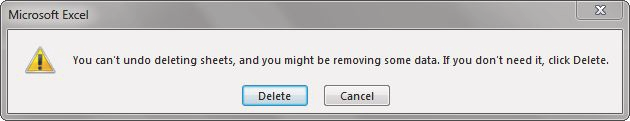
\includegraphics[width=\maxwidth{.95\linewidth}]{gfx/ch06_fig03}
	\caption{Warning Message Box}
	\label{06:fig03}
\end{figure}

\subsection{Grouping and Ungrouping Sheets}

Take a look at the monthly sheets again. Notice that there is a place in each of these sheets to calculate three pieces of Summary data: Income, Expenses, and Balance; but there are no formulas in these cells. There is also a place for the \% of Income Spent, but a formula is needed in \fmtCellLocation{I6:I7} to calculate this. If these formulas were individually added in each of the $ 12 $ month sheets, it would take a long time and since this task is very repetitive it would also be likely that mistakes would be made along the way. By grouping all the month sheets together, the formulas are entered only once but appear in all the sheets.

\begin{enumerate}
	\item Click on the \fmtWorksheetName{January} sheet to make it active.
	\item Hold the \fmtKeystroke{Shift} key down and click on the \fmtWorksheetName{December} sheet.
\end{enumerate}

Now all $ 12 $ sheets should be selected. This can be verified in two ways: the sheet tabs that have been selected are in bold font at the bottom of the screen and the title bar at the top of the screen adds the word \textit{[Group]} to the end of the title. These are both visible of these in Figure \ref{06:fig04}.

\begin{figure}[H]
	\centering
	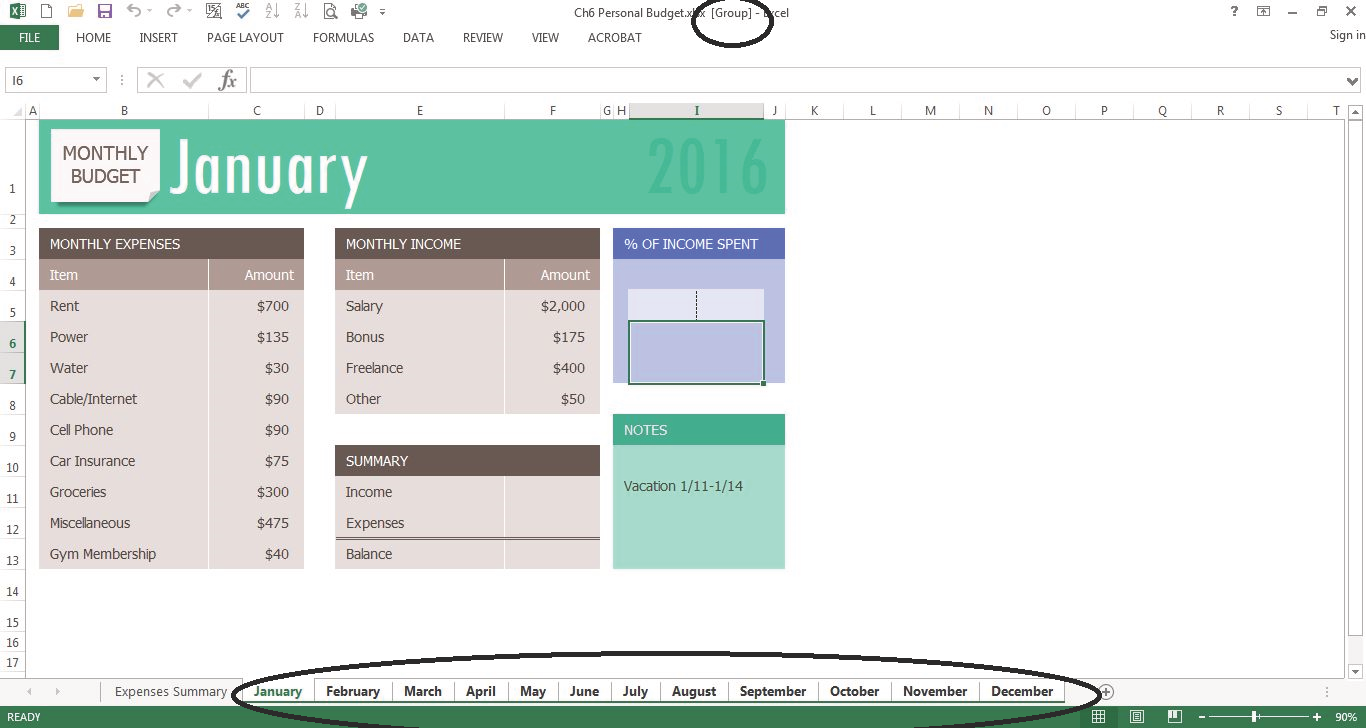
\includegraphics[width=\maxwidth{.95\linewidth}]{gfx/ch06_fig04}
	\caption{Grouped Sheets}
	\label{06:fig04}
\end{figure}

\textit{It is important to remember that any changes made to the January sheet will be made to all of the grouped sheets.} This makes it easy to make changes to all the sheets at once, but they must be ungrouped after making changes or data on linked sheets can be inadvertently destroyed. 

\begin{enumerate}
	\item Click in \fmtCellLocation{F11} in the \fmtWorksheetName{January} grouped sheet.
	\item Enter the formula \fmtTyping{=SUM(F5:F8)}.
	\item In \fmtCellLocation{F12}, enter the formula \fmtTyping{=SUM(C5:C13)}.
	\item In \fmtCellLocation{F13}, subtract Expenses from Income. In the \fmtWorksheetName{January} sheet, the balance should be $ \$690 $. \textit{Hint}: if the answer is negative, then Income was subtracted from Expenses.
	\item Click on \fmtCellLocation{I6}. (\fmtCellLocation{I6} and \fmtCellLocation{I7} are formatted and merged together, this is fine.)
	\item Enter a formula that divides Expenses (\fmtCellLocation{F12}) by Income (\fmtCellLocation{F11}). The answer will show as a percentage since this cell has already been formatted to do this. \textit{Hint}: If the percentage is greater than 100\% the numbers are reversed.
\end{enumerate}

Notice that a data bar was set up in \fmtCellLocation{I5} to visually show the income spent, which is a skill that was covered elsewhere in the course. The \fmtWorksheetName{January} sheet should now look like Figure \ref{06:fig05}.

\begin{figure}[H]
	\centering
	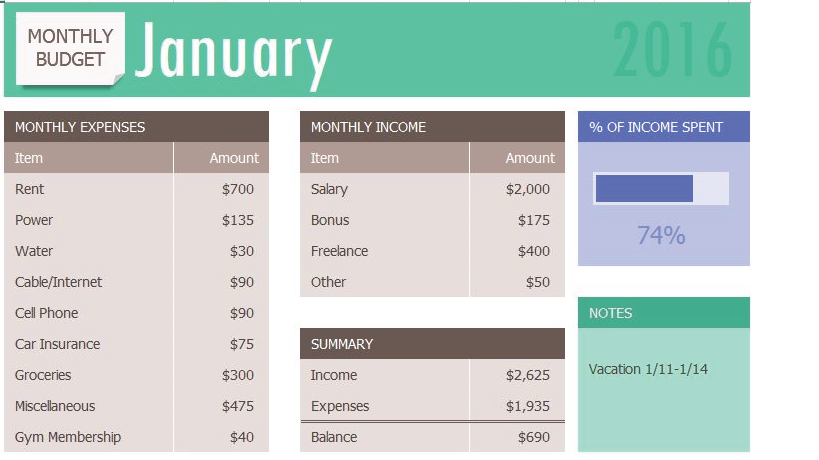
\includegraphics[width=\maxwidth{.95\linewidth}]{gfx/ch06_fig05}
	\caption{January Sheet with Formulas}
	\label{06:fig05}
\end{figure}

\begin{enumerate}[resume]
	\item Now that the monthly sheets are done, they need to be ungrouped. Right-click on one of the grouped sheets and choose \fmtPopupButton{Ungroup Sheets}. Notice the sheets tabs are no longer bold and the word \textit{[Group]} is no longer in the title bar.
	\item Click on several of the month sheets to see that all the formulas have been added.
	\item Click on the \fmtWorksheetName{December} sheet. The sheet should now look like Figure \ref{06:fig06}.
\end{enumerate}

\begin{figure}[H]
	\centering
	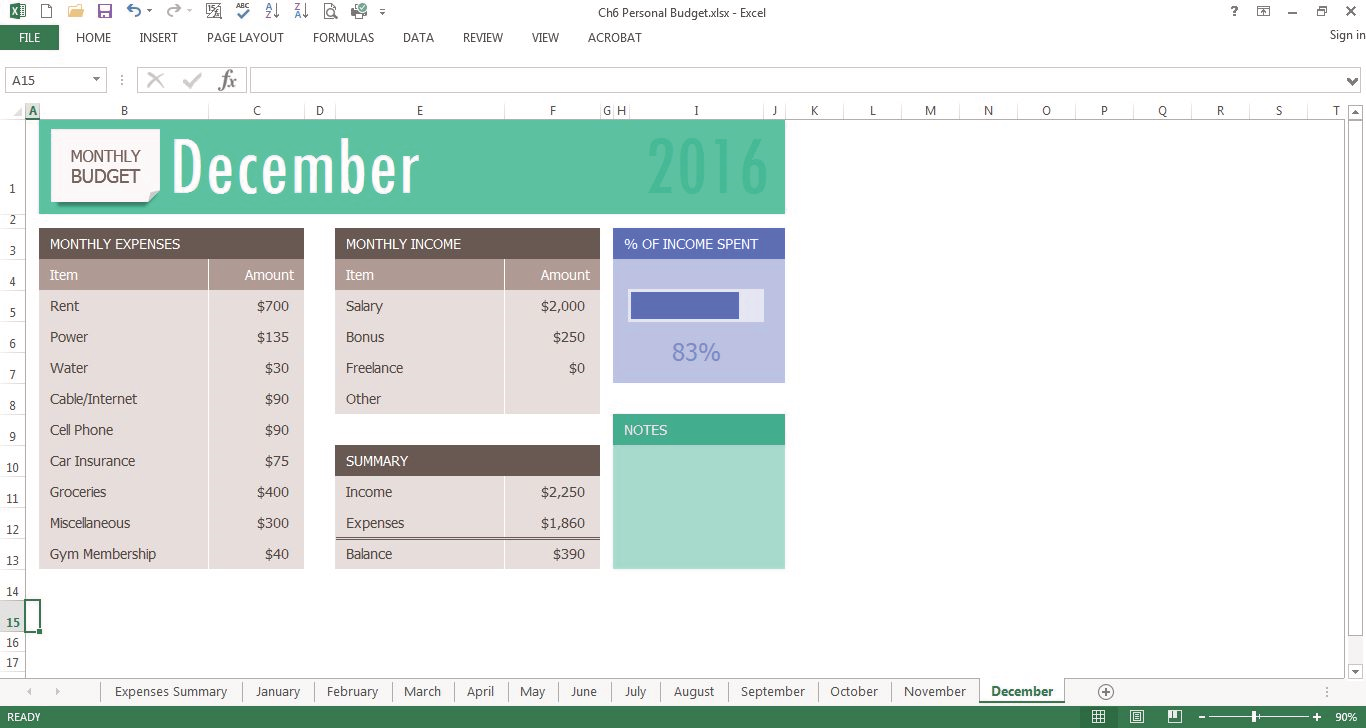
\includegraphics[width=\maxwidth{.95\linewidth}]{gfx/ch06_fig06}
	\caption{December Sheet with Formulas}
	\label{06:fig06}
\end{figure}

\begin{enumerate}
	\item Take a look at the Notes in the \fmtWorksheetName{September} sheet. It says that the rent was raised in September, so the Gym Membership needs to be cancelled and $ \$0 $ should be entered for the Gym amount in October, November, and December.
	\item Group the \fmtWorksheetName{October}, \fmtWorksheetName{November}, and \fmtWorksheetName{December} sheets. If this is done successfully these three sheet names should be bold and the word \textit{[Group]} will appear in the Title bar.
	\item Click on \fmtCellLocation{C13} and change the amount to $ \$0 $. Press \fmtKeystroke{Enter}.
	\item Ungroup the sheets.The balances should be October: \$605, November: \$530, and December: $ \$430 $.
\end{enumerate}

\begin{center}
	\begin{sklbox}{Skill Refresher}
		\textbf{To Group Sheets}
		\\
		\begin{itemize}
			\setlength{\itemsep}{0pt}
			\setlength{\parskip}{0pt}
			\setlength{\parsep}{0pt}
			
			\item Click on the leftmost sheet group; then hold the \fmtKeystroke{Shift} key down and click on the rightmost sheet to group.
		\end{itemize}
			
		\bigskip
			
		\textbf{To Ungroup Sheets}
		\begin{itemize}
			\setlength{\itemsep}{0pt}
			\setlength{\parskip}{0pt}
			\setlength{\parsep}{0pt}
			
			\item Right-click on one of the grouped sheets and choose \fmtRibbonButton{Ungroup Sheets}.
		\end{itemize}
	\end{sklbox}
\end{center}

\begin{center}
	\begin{tkwbox}{Key Take-Aways}
		\textbf{Worksheets}
		\\
		\begin{itemize}
			\setlength{\itemsep}{0pt}
			\setlength{\parskip}{0pt}
			\setlength{\parsep}{0pt}
			
			\item Sheets can be easily moved, copied, deleted, and renamed.
			\item When grouped, identically formatted sheets can be changed at the same time.
			
		\end{itemize}
	\end{tkwbox}
\end{center}

\section{Formulas With 3-D References}

\begin{center}
	\begin{objbox}{Learning Objectives}
		\begin{itemize}
			\setlength{\itemsep}{0pt}
			\setlength{\parskip}{0pt}
			\setlength{\parsep}{0pt}

			\item Entering formulas that reference another sheet.
			\item Using the SUM function to total values on multiple sheets.
			
		\end{itemize}
	\end{objbox}
\end{center}

The \fmtWorksheetName{Summary} sheet in many multiple sheet workbooks is utilized to present totaled information from the other sheets in the file. This is done to give a quick synopsis of all the other sheets in one convenient location. For this reason, the \fmtWorksheetName{Summary} sheet is usually the first sheet in multiple-sheet files. Summary sheets ``pull'' data from the other sheets using three-dimensional (3-D) cell references. In order to distinguish between \fmtCellLocation{A3} in the \fmtWorksheetName{Summary} sheet, \fmtCellLocation{A3} in the \fmtWorksheetName{January} sheet, \fmtCellLocation{A3} in the \fmtWorksheetName{February} sheet, etc.; a 3-D cell reference includes the sheet name along with the cell reference. The syntax to reference a cell in a different sheet is \fmtTyping{=SheetName!CellRange}. So, the cell reference for \fmtCellLocation{A15} in the \fmtWorksheetName{March} sheet would be \fmtTyping{=March!A15}.

\begin{center}
	\begin{infobox}{Best Practice}
		\textbf{Summary Sheet}
		\\
		\\
		Even if there are no 3-D formulas to summarize on a summary sheet, it is considered a best practice to include a summary sheet with information about the data contained in the workbook and contact information for the person who created the workbook.  
	\end{infobox}
\end{center}

Start working on the \fmtWorksheetName{Summary} sheet by trying out some 3-D formula.

\begin{enumerate}
	\item Click on the \fmtWorksheetName{Expenses Summary} sheet tab at the bottom of the screen.
	\item Click on \fmtCellLocation{C5} and enter the formula \fmtTyping{=January!C5}. Press \fmtKeystroke{Enter}. This will get the amount $ \$700 $ from cell \fmtCellLocation{C5} in the \fmtWorksheetName{January} sheet.
	\item Delete the formula in \fmtCellLocation{C5} in the \fmtWorksheetName{Expenses Summary} sheet.
	\item This time, click on \fmtCellLocation{C5} and type \fmtTyping{=}. Then click on the \fmtWorksheetName{January} sheet, and then click on \fmtCellLocation{C5}.
	\item Press \fmtKeystroke{Enter}. This will put the same formula, \fmtTyping{=January!C5}, in cell \fmtCellLocation{C5} in the \fmtWorksheetName{Expenses Summary} sheet and will return the value $ \$700 $.
	\item In cell \fmtCellLocation{C6} in the \fmtWorksheetName{Expenses Summary} sheet, try entering a formula for the Power amount in the \fmtWorksheetName{April} sheet. The Power amount should be $ \$135 $.
	\item Delete the formulas in cells \fmtCellLocation{C5} and \fmtCellLocation{C6} in the \fmtWorksheetName{Expenses Summary} sheet.
\end{enumerate}

For the Annual Amounts in \fmtCellLocation{C5:C13} in the \fmtWorksheetName{Expenses Summary} sheet, the amount from a single month's sheet is not needed; instead, the sum of all the entries in all the monthly sheets should be entered. So, a three-dimensional sum for all twelve month sheets should be entered. Here is a helpful hint on the steps to follow to add through multiple sheets.

\begin{center}
	\begin{sklbox}{Skill Refresher}
		\textbf{To SUM across sheets}
		\\
		\begin{itemize}
			\setlength{\itemsep}{0pt}
			\setlength{\parskip}{0pt}
			\setlength{\parsep}{0pt}
			
			\item Click on the cell where the 3-D SUM should appear.
			\item Type \fmtTyping{=SUM(}
			\item Click on the leftmost sheet in the group of sheets to sum.
			\item Hold the \fmtKeystroke{Shift} key down and click on the rightmost sheet in the group of sheets to sum.
			\item Click on the cell in the sheet that should be summed.
			\item Press \fmtKeystroke{Enter}.
			
		\end{itemize}
	\end{sklbox}
\end{center}

Follow these steps to sum all of the monthly amounts in the \fmtWorksheetName{Expenses Summary} sheet.

\begin{enumerate}
	\item Click in \fmtCellLocation{C5} in the \fmtWorksheetName{Expenses Summary} sheet.
	\item Type \fmtTyping{=SUM(}. (Make sure to type the open parentheses.)
	\item Click on the \fmtWorksheetName{January} sheet.
	\item Hold the \fmtKeystroke{Shift} key down and click on the \fmtWorksheetName{December} sheet.
	\item Click on \fmtCellLocation{C5} again and press \fmtKeystroke{Enter}. Cell \fmtCellLocation{C5} should display the sum of $ \$8,400 $.
	\item Click on \fmtCellLocation{C5} in the \fmtWorksheetName{Expenses Summary} sheet. The formula bar should show the following: \fmtTyping{=SUM(January:December!C5)}. This means Excel should calculate the sum of \fmtCellLocation{C5} in the sheets \fmtWorksheetName{January} through \fmtWorksheetName{December}.
	\item For another 3-D sum, click on \fmtCellLocation{C6}.
	\item Type \fmtTyping{=SUM(}. (Make sure to type the open parentheses.)
	\item Click on the \fmtWorksheetName{January} sheet.
	\item Hold the \fmtKeystroke{Shift} key down and click on the \fmtWorksheetName{December} sheet.
	\item Click on \fmtTyping{C6} again and press \fmtKeystroke{Enter}. Cell \fmtCellLocation{C6} should now display the sum of $ \$1,610 $.
	\item Click on \fmtCellLocation{C6} in the \fmtWorksheetName{Expenses Summary} sheet. The formula bar should show the following: \fmtTyping{=SUM(January:December!C6)}.
\end{enumerate}

Copy \fmtCellLocation{C6} down through \fmtCellLocation{C13} to fill in the rest of the formulas. The \fmtWorksheetName{Expenses Summary} sheet should match Figure \ref{06:fig07}.

\begin{figure}[H]
	\centering
	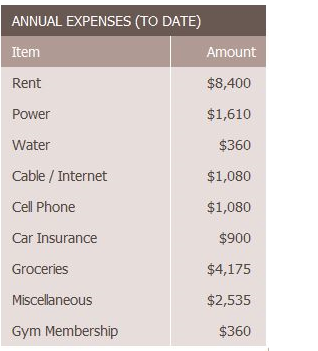
\includegraphics[width=\maxwidth{.95\linewidth}]{gfx/ch06_fig07}
	\caption{Complete Expenses Summary Formulas}
	\label{06:fig07}
\end{figure}

While the 3-D formulas are complete in the \fmtWorksheetName{Expenses Summary} sheet, the summary feels like it is lacking something. Add a visual representation of the summary numbers to the sheet.

\begin{enumerate}
	\item Highlight cells \fmtCellLocation{B5:C13} in the \fmtWorksheetName{Expenses Summary} sheet.
	\item Click on \fmtRibbonButton{Pie Chart} in the \fmtRibbonTab{Insert} tab in the ribbon and select the \fmtPopupButton{2-D pie}.
	\item Move and resize the pie chart so that it fills cells \fmtCellLocation{D3:J15}.
	\item Delete the chart title.
	\item Move the legend to the right side of the chart. Resize the legend as needed.
	\item Add percentage data labels to the pie slices. Format the data labels to be bold with white font color. The complete \fmtWorksheetName{Expenses Summary} sheet should look like Figure \ref{06:fig08} below.
	\item Save the workbook. 
	\item If it is necessary to print the assignment, print ONLY the Summary sheet in both regular and formula view. 
	\item Close the workbook.
\end{enumerate}

\begin{figure}[H]
	\centering
	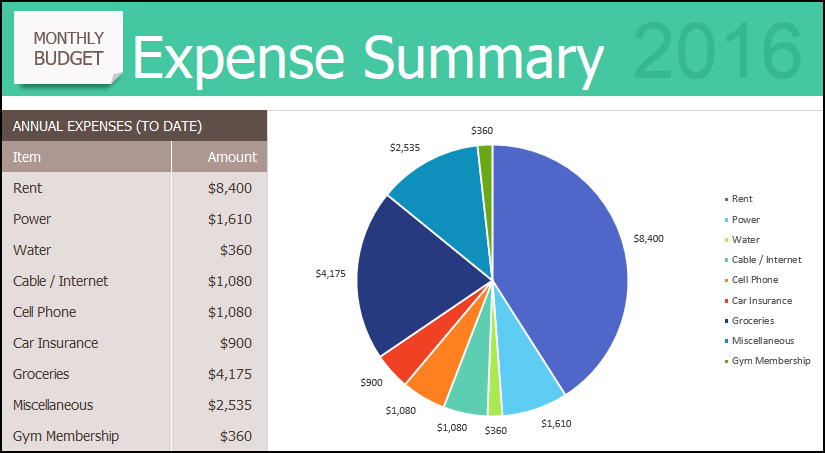
\includegraphics[width=\maxwidth{.95\linewidth}]{gfx/ch06_fig08}
	\caption{Completed Expenses Summary Sheet}
	\label{06:fig08}
\end{figure}

\begin{center}
	\begin{sklbox}{Skill Refresher}
		\textbf{3-D References in Formulas}
		\\
		\begin{itemize}
			\setlength{\itemsep}{0pt}
			\setlength{\parskip}{0pt}
			\setlength{\parsep}{0pt}
			
			\item To reference a cell in another sheet, use the formula syntax \fmtTyping{=SheetName!CellAddress}.
			\bigskip
			\item To enter a 3-D reference:

			\begin{enumerate}
				\item Click on the cell where the formula should appear and type \fmtTyping{=}.
				\item Click on the sheet with the cell to reference.
				\item Click on the cell in the sheet and press \fmtKeystroke{Enter}.
			\end{enumerate}
			
		\end{itemize}
	\end{sklbox}
\end{center}

\begin{center}
	\begin{tkwbox}{Key Take-Aways}
		\textbf{3-D References}
		\\
		\begin{itemize}
			\setlength{\itemsep}{0pt}
			\setlength{\parskip}{0pt}
			\setlength{\parsep}{0pt}
			
			\item 3-D references in formulas allow data from one or more sheets to be used on another sheet.
			
		\end{itemize}
	\end{tkwbox}
\end{center}

\section{Templates}

\begin{center}
	\begin{objbox}{Learning Objectives}
		\begin{itemize}
			\setlength{\itemsep}{0pt}
			\setlength{\parskip}{0pt}
			\setlength{\parsep}{0pt}

			\item Use an existing Microsoft Excel template to create a new spreadsheet.
			\item Create a custom template that can be used to create new spreadsheets.
		
		\end{itemize}
	\end{objbox}
\end{center}

A template is a predefined pattern for a spreadsheet. Hundreds of templates created by Microsoft are available to use inside Excel and these templates are very helpful to quickly start and complete a new task in Excel. Templates include all the formulas, formatting, etc. needed in a professional Excel spreadsheet. All that is left to do is enter the data. Predefined Microsoft templates include everything from billing statements to blood pressure trackers to business cards. Categories include: Business, Personal, Industry, Financial Management, Logs, Calculators, and Lists.

Sometimes a very specific template is needed that has not already been created by Microsoft. Taking the time to create a custom template allows users to create new spreadsheets from it over and over again. If a new version of some spreadsheet is needed on a regular basis, templates will make this work much easier. This chapter explores both types of templates: predefined and custom.

\subsection{Predefined Templates}

Microsoft has made many predefined templates available in Excel. Follow these steps to explore this resource.

\begin{enumerate}
	\item Click the \fmtRibbonTab{File} tab in the ribbon.
	\item Click \fmtPopupButton{New} in the Backstage View.
	\item Click in the \fmtPopupBox{Search} box for Online template.
	\item Type \fmtTyping{Travel} and press \fmtKeystroke{Enter}.
	\item Click on the \fmtPopupButton{Travel Expense Report} and click \fmtPopupButton{Create}. Note: If this template is not available, ask the instructor which template to use.
\end{enumerate}

The screen should look like Figure \ref{06:fig09} below. Notice the design, layout, and formulas have already been set up.

\begin{figure}[H]
	\centering
	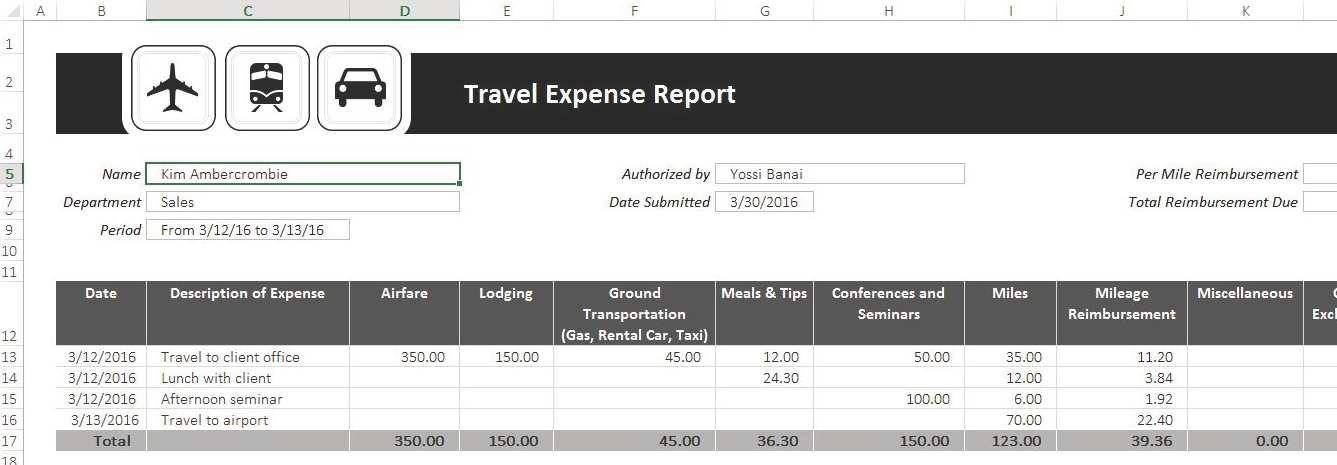
\includegraphics[width=\maxwidth{.95\linewidth}]{gfx/ch06_fig09}
	\caption{Travel Expenses Report Template}
	\label{06:fig09}
\end{figure}

Complete the following steps to investigate this template.

\begin{enumerate}
	\item Change the Name to anything appropriate.
	\item Change the Department to CAS.
	\item Press \fmtKeystroke{Ctrl}$+$\fmtKeystroke{$ \sim $} (that is \textit{Ctrl+tilde}) to see where the formulas are in the sheet. Working in the formula view helps find formulas, so they will not be accidentally deleted.
	\item In formula view, carefully delete just the data. Do not delete any formulas!
	\item Press \fmtKeystroke{Ctrl}$+$\fmtKeystroke{$ \sim $} (that is \textit{Ctrl+tilde}) again to return to Normal view.
	\item Enter dates and expenses for an imaginary trip in the first three rows under the column headings.
	\item Save the completed file as \fmtWorkbookName{CH6 Travel Expenses}. Close the file.
\end{enumerate}

\begin{center}
	\begin{sklbox}{Skill Refresher}
		\textbf{Predefined Template}
		\\
		\begin{itemize}
			\setlength{\itemsep}{0pt}
			\setlength{\parskip}{0pt}
			\setlength{\parsep}{0pt}

			\item Click on the \fmtRibbonTab{File} tab in the ribbon.
			\item Click on \fmtRibbonButton{New}
			\item Type the desired template description in the Search box, and press \fmtKeystroke{Enter}.
			
		\end{itemize}
	\end{sklbox}
\end{center}

\subsection{Custom Templates}

To create a custom template a blank template can be created or an existing spreadsheet can be saved as a template. Either way, the template can be used to create new spreadsheets that have a uniform appearance and set of functions. For this exercise, the existing \fmtWorkbookName{CH6 Personal Budget} file will be converted into a template but the assignments at the end of the chapter a build a template from scratch.

\begin{enumerate}
	\item Open the \fmtWorkbookName{CH6 Personal Budget.xlsx} file.
	\item Group the month sheets (\fmtWorksheetName{January} through \fmtWorksheetName{December}).
	\item Press \fmtKeystroke{Ctrl}$+$\fmtKeystroke{$ \sim $} (that is \textit{Ctrl+tilde}) to switch to Formula view.
	\item Delete only the data from these sheets, not labels or formulas. The only data is in \fmtCellLocation{C5:C13}, \fmtCellLocation{F5:F8}, and in the Notes in \fmtCellLocation{H11:J13}.
	\item Highlight \fmtCellLocation{C5:C13} (with all the sheets still grouped) and press \fmtKeystroke{Delete}.
	\item Highlight \fmtCellLocation{F5:F8} (with all the sheets still grouped) and press \fmtKeystroke{Delete}.
	\item Highlight \fmtCellLocation{H11:J13} (with all the sheets still grouped) and press \fmtKeystroke{Delete}.
	\item Press \fmtKeystroke{Ctrl}$+$\fmtKeystroke{$ \sim $} (that is \textit{Ctrl+tilde}) to switch back to Normal view.
	\item Ungroup the sheets. 
	\item Look through the sheets to check that only the data has been deleted. Notice the error message \textit{\#DIV/O} appears in \fmtCellLocation{I6:I7} since the data for this formula has been deleted. The \fmtWorksheetName{January} sheet should look like Figure \ref{06:fig10}.
\end{enumerate}

\begin{figure}[H]
	\centering
	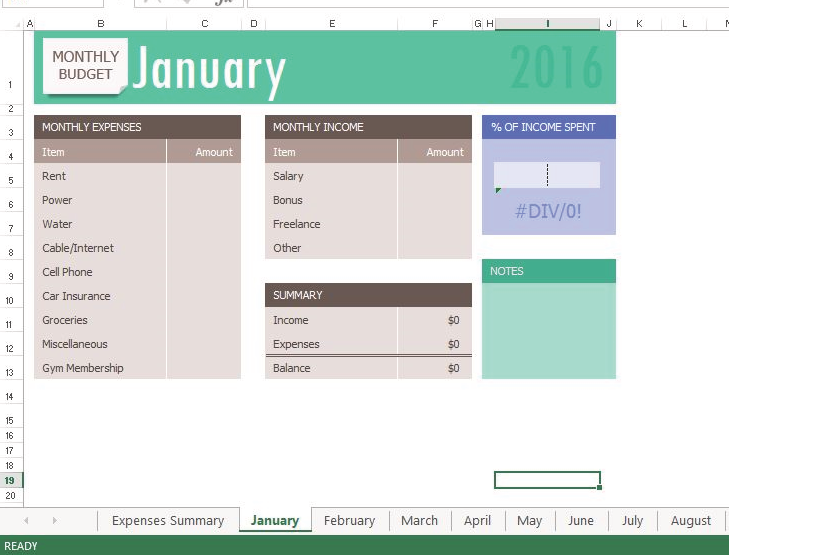
\includegraphics[width=\maxwidth{.95\linewidth}]{gfx/ch06_fig10}
	\caption{January Template Sheet}
	\label{06:fig10}
\end{figure}

\textit{Note}: There are only formulas and the pie chart in the \fmtWorksheetName{Expenses Summary} sheet, so nothing needs to be deleted from this sheet to setup the template.

\begin{enumerate}
	\item Click the \fmtRibbonTab{File} tab in the ribbon and then click \fmtRibbonButton{Save As}.
	\item Choose the location to save the file.
	\item In the \fmtPopupBox{Save as type} pull-down list, select \fmtPopupButton{Excel Template (*.xltx)}.
	\item At the top of the screen, double-check that the location selected to save the file has not changed. If it has, use the pull-down list to find the location to save the file. \textit{Be Careful Here!} By default, Excel will try to save this to a default template file location on the local hard drive.
	\item Type in the file name \fmtWorkbookName{CH6 Personal Budget Template.xltx}. Carefully compare the screen with Figure \ref{06:fig11}. Keep in mind that the template file may be getting saved to a different place on the computer since Excel will normally save templates to a specific folder on the local hard drive.
	\item Click \fmtPopupButton{Save}.
\end{enumerate}

\begin{figure}[H]
	\centering
	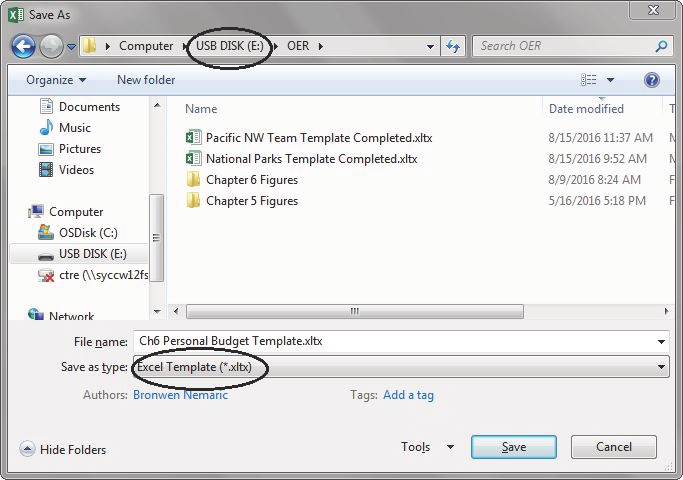
\includegraphics[width=\maxwidth{.95\linewidth}]{gfx/ch06_fig11}
	\caption{Save As Template}
	\label{06:fig11}
\end{figure}

\begin{center}
	\begin{sklbox}{Skill Refresher}
		\textbf{Save a Template}
		\\
		\begin{itemize}
			\setlength{\itemsep}{0pt}
			\setlength{\parskip}{0pt}
			\setlength{\parsep}{0pt}

			\item Click the \fmtRibbonTab{File} tab in the ribbon and then click \fmtRibbonButton{Save As}.
			\item Choose the location to save the file.
			\item In the \fmtPopupBox{Save as type} pull-down list, select \fmtPopupButton{Excel Template (*.xltx)}.
			\item At the top of the screen, double-check that the location to save the file to has not changed. If it has, use the pull-down list to find the location to save the file. \textit{Be Careful Here!} By default, Excel will save templates to a default file location on the local hard drive.
			\item Enter the file name.
			\item Click \fmtPopupButton{Save}.
			
		\end{itemize}
	\end{sklbox}
\end{center}

Use the new budget template to start a Personal Budget file for $ 2017 $. Use the \fmtWorkbookName{Ch6 Personal Budget Template} to create the new file, but do not overwrite the template since it will be used to create budget files in future years. To do this, save the file to the new $ 2017 $ file name before filling in any data.

\begin{enumerate}
	\item With the \fmtWorkbookName{CH6 Personal Budget Template} open, click the \fmtRibbonTab{File} tab in the ribbon.
	\item Choose \fmtRibbonButton{Save As} and choose the location to save the $ 2017 $ version of the file.
	\item Change the \fmtPopupBox{Save as Type} back to \fmtPopupButton{Excel Workbook (*.xlsx)}.
	\item Enter the File name \fmtWorkbookName{CH6 2017 Personal Budget}. Compare the screen to Figure \ref{06:fig12}.
\end{enumerate}

\begin{figure}[H]
	\centering
	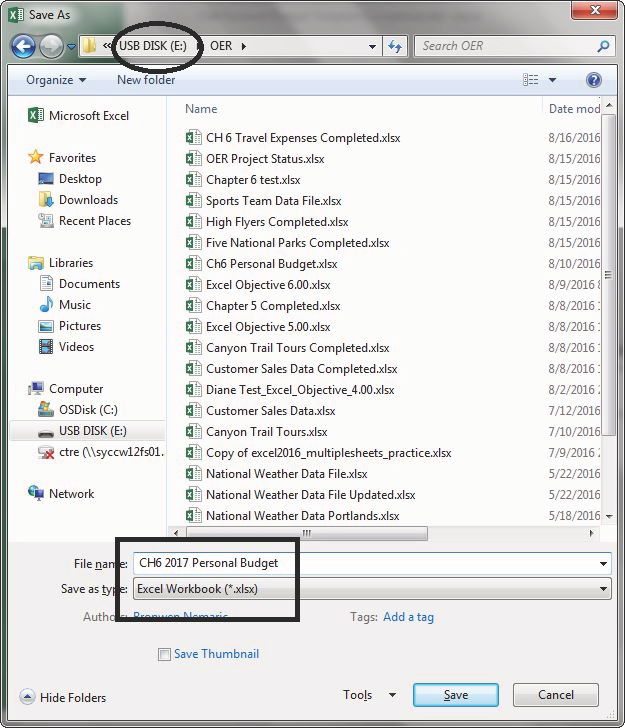
\includegraphics[width=\maxwidth{.95\linewidth}]{gfx/ch06_fig12}
	\caption{Save As 2017 Budget File}
	\label{06:fig12}
\end{figure}

\begin{enumerate}[resume]
	\item Click \fmtPopupButton{Save}.
	\item Group all the sheets together including the \fmtWorksheetName{Expenses Summary} sheet.
	\item Click on \fmtCellLocation{H1}. Type $ 2017 $ and press \fmtKeystroke{Enter}.
	\item Ungroup the sheets.
	\item Click on the \fmtWorksheetName{January} sheet. Enter the data found in Figure \ref{06:fig13}.
\end{enumerate}

\begin{figure}[H]
	\centering
	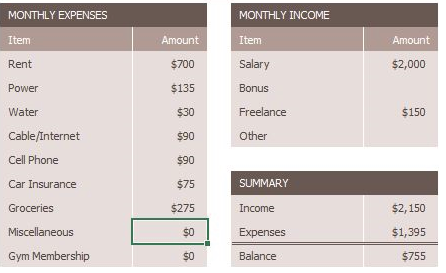
\includegraphics[width=\maxwidth{.95\linewidth}]{gfx/ch06_fig13}
	\caption{January 2017 Data}
	\label{06:fig13}
\end{figure}

\begin{enumerate}[resume]
	\item Click on the \fmtWorksheetName{Expenses Summary} sheet. The data and the pie chart should show the January data since that is the only data in the twelve month sheets for now. The sheet should look like Figure \ref{06:fig14}.
\end{enumerate}

\begin{figure}[H]
	\centering
	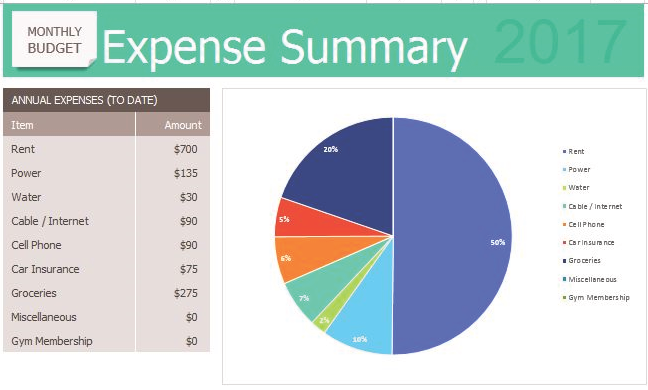
\includegraphics[width=\maxwidth{.95\linewidth}]{gfx/ch06_fig14}
	\caption{Expense Summary Sheet}
	\label{06:fig14}
\end{figure}

\begin{enumerate}[resume]
	\item Save the file.
\end{enumerate}

\begin{center}
	\begin{tkwbox}{Key Take-Aways}
		\textbf{Templates}
		\\
		\begin{itemize}
			\setlength{\itemsep}{0pt}
			\setlength{\parskip}{0pt}
			\setlength{\parsep}{0pt}
			
			\item Templates save time and effort when compared to designing and creating spreadsheets files from scratch.
			\item There are many predefined templates in Excel.
			\item Custom templates can be created for special purposes.
			
		\end{itemize}
	\end{tkwbox}
\end{center}

\section{Preparing to Print}

\begin{center}
	\begin{objbox}{Learning Objectives}
		\begin{itemize}
			\setlength{\itemsep}{0pt}
			\setlength{\parskip}{0pt}
			\setlength{\parsep}{0pt}
			
			\item Printing all of the worksheets in a workbook at one time.
			\item Preparing multiple worksheets for printing using grouping.
			
		\end{itemize}
	\end{objbox}
\end{center}

Just like consistency in formatting is important when working with workbooks containing multiple worksheets with the same type of data, so is consistency in page setup. Now that the \fmtWorkbookName{Personal Budget 2017} workbook is complete, prepare it for printing by changing the page orientation and adding a header. All $ 13 $ worksheets will also be printed at one time.

\subsection{Applying Page Setup Options to Grouped Worksheets}

\textit{Data file: CH6 2017 Personal Budget.}

As always, review the workbook in Print Preview before considering it complete. When checking this workbook, notice that the worksheets are each printing on two pages. Switch all the worksheets to Landscape orientation to see if that helps. Also add a footer with the worksheet name to each of the worksheets.

\begin{enumerate}
	\item Go to \fmtPopupBox{Print Preview}. To view all of the worksheets at one time, select \fmtPopupButton{Print Entire Workbook} in the first box in the Settings section. There should be $ 26 $ pages to scroll through in Print Preview. At this point, clicking the \fmtPopupButton{Print} button would print all of the worksheets rather than just the active sheet.
	\item Exit Backstage View. The page orientation of all the sheets can be changed at one time, but not in Print Preview.
	\item Group all of the worksheets together, including the \fmtWorksheetName{Expenses Summary} sheet through the \fmtWorksheetName{December} sheet.
	\item Click on the \fmtRibbonTab{Page Layout} tab on the ribbon, then select \fmtRibbonButton{Landscape} using the Orientation button in the \fmtRibbonGroup{Page Setup} group.
	\item Click the \fmtRibbonButton{Page Setup} dialog box launcher arrow in the \fmtRibbonGroup{Page Setup} group then click the \fmtPopupButton{Header/Footer} tab.
	\item Click the \fmtPopupButton{Custom Footer} button. In the center section, insert the worksheet name using the \fmtPopupButton{Insert Sheet Name} button. The Footer dialog box should look like Figure \ref{06:fig15}.
	\item Click \fmtPopupButton{OK} to close the \fmtPopupBox{Footer} dialog box. Click \fmtPopupButton{OK} again to close the \fmtPopupBox{Page Setup} dialog box.
	\item Return to Print Preview to confirm that each worksheet is printing on one page, in landscape orientation, with the correct worksheet name appearing in the footer.
\end{enumerate}

\begin{figure}[H]
	\centering
	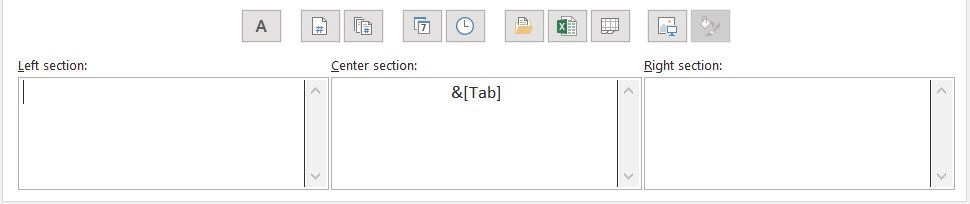
\includegraphics[width=\maxwidth{.95\linewidth}]{gfx/ch06_fig15}
	\caption{Insert Worksheet Name}
	\label{06:fig15}
\end{figure}

Print Preview makes it clear that the \fmtWorksheetName{Expenses Summary} sheet is not set to print correctly. Part of the chart is appearing on a second page. This can be easily fixed by changing the Scaling, but to change the scaling of only the \fmtWorksheetName{Expenses Summary} sheet, not the entire workbook, the worksheets need to be ungrouped.

\begin{enumerate}
	\item Exit Backstage View.
	\item Ungroup the worksheets by right-clicking on any of the worksheet tabs and selecting \fmtPopupButton{Ungroup Sheets}.
	\item If needed, click on the \fmtWorksheetName{Expenses Summary} worksheet tab to make it the active worksheet.
	\item Click on the \fmtRibbonTab{Page Layout} tab on the ribbon and locate the \fmtRibbonGroup{Scale to Fit} group of commands. (See Figure  \ref{06:fig16})
\end{enumerate}

\begin{figure}[H]
	\centering
	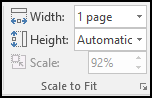
\includegraphics[width=\maxwidth{.95\linewidth}]{gfx/ch06_fig16}
	\caption{Scale to Fit}
	\label{06:fig16}
\end{figure}

\begin{enumerate}
	\item Click the drop-down arrow for \fmtPopupButton{Width:} and select $ 1 $ page. This has the same result as selecting \fmtPopupButton{Fit All Columns on One Page} in the \fmtPopupBox{Scaling} setting in Print Preview.
	\item Return to Print Preview to confirm that the \fmtWorksheetName{Expenses Summary} worksheet is now printing on one page only.
	\item Exit Backstage View.
	\item Save the \fmtWorkbookName{CH6 2017 Personal Budget} workbook.
	\item Compare the workbook with the self-check answer keys (found in the Course Files) and then submit the following files as directed by the instructor.
	
	\begin{itemize}
		\item \fmtWorkbookName{CH6 Personal Budget}
		\item \fmtWorkbookName{CH6 Personal Budget Template}
		\item \fmtWorkbookName{CH6 Travel Expenses}
		\item \fmtWorkbookName{CH6 2017 Personal Budget}
	\end{itemize}

\end{enumerate}

\begin{center}
	\begin{tkwbox}{Key Take-Aways}
		\textbf{Printing}
		\\
		\begin{itemize}
			\setlength{\itemsep}{0pt}
			\setlength{\parskip}{0pt}
			\setlength{\parsep}{0pt}
			
			\item To print all of the worksheets in a workbook at one time select \fmtPopupButton{Print Entire Workbook} in the \fmtPopupBox{Print Settings}.
			\item Page setup options, such as scaling, orientation, and headers/footers, can be applied to multiple worksheets at one time by grouping them.
			
		\end{itemize}
	\end{tkwbox}
\end{center}

\section{Chapter Practice}

\subsection{A Multiple Sheet Template for a Sports Team}

\textit{Data file: PR6 Data}

The coaches of the \textit{Pacific Northwest Soccer Club} want a consistent way to keep track of their team statistics. To help with this, create a template for season stats for each team. The \textit{High Flyers} team coach will use the template to enter that team's statistics into a spreadsheet.

\begin{enumerate}
	\item Open the data file \fmtWorkbookName{PR6 Data} and save the file as \fmtWorkbookName{PR6 Pacific NW Sports Team}.
	\item Copy the range \fmtCellLocation{B11:G22} in the \fmtWorksheetName{Season Stats} sheet to the same range in the \fmtWorksheetName{Player Stats} sheet.
	\item Group the sheets and add the following formulas to both sheets.

	\begin{itemize}
		\item In \fmtCellLocation{C22} and \fmtCellLocation{D22}, count the \textit{Xs} in rows $ 12 $ through $ 21 $. To do this, use a \fmtTyping{COUNTA} formula.
		\item In \fmtCellLocation{E22} and \fmtCellLocation{F22}, sum rows $ 12 $ through $ 21 $.
		\item In \fmtCellLocation{G12}, calculate Goal Percentage by dividing the number of Shots by the number of Goals. This will display an error message because there are zeros in column F. An \fmtTyping{IF} statement that tests the value of column F will keep error messages from appearing. Change the formula in \fmtCellLocation{G12} with the following three pieces.
		\begin{itemize}
			\item Test: is \fmtCellLocation{F12} greater than zero
			\item If the Test is True: divide the number of Goals by the number of Shots
			\item If the Test is False: enter a zero
		\end{itemize}
		\item Copy \fmtCellLocation{G12} down the column through \fmtCellLocation{G22}. Format these cells as percentages.
		\item For an extra challenge, put the ``banded row'' format back in \fmtCellLocation{G12:G22}.
		\end{itemize}	
	
	\item Ungroup the sheets.
	\item Save the file as a template called \fmtWorkbookName{PR6 Pacific NW Team Template.xltx}. Make sure to save the  template to a USB drive and not the default folder for templates on the local hard drive.
	\item Make a new file using the \fmtWorkbookName{PR6 Pacific NW Team Template} and save it as \fmtWorkbookName{PR6 High Flyers.xlsx}.
	\item In the \fmtWorksheetName{Season Stats} sheet, enter the following data:
	
	\begin{itemize}
		\item \fmtCellLocation{D3} – High Flyers
		\item \fmtCellLocation{D4} – Fall and the current year (\ie – Fall 2020)
		\item \fmtCellLocation{D5} – Pacific Northwest Soccer
	\end{itemize}
	
	\item Make up a coach's name, phone number, and email address for row $ 8 $.
	\item Make four copies of the \fmtWorksheetName{Player Statistics} sheet. Rename the player sheets \fmtWorksheetName{Player 1}, \fmtWorksheetName{Player 2}, \fmtWorksheetName{Player 3}, \fmtWorksheetName{Player 4}, and \fmtWorksheetName{Player 5}.
	\item Group the Player sheets and enter the following formulas.

	\begin{itemize}
		\item A formula in \fmtCellLocation{D4} that points to cell \fmtCellLocation{D3} in the \fmtWorksheetName{Season Stats} sheet. \textit{Note}: the formula will be \fmtTyping{='Season Stats'!D3:G3} instead of \fmtTyping{='Season Stats'!D3} because \fmtCellLocation{D3:G3} are merged together.
		\item A formula in \fmtCellLocation{D5} that points to cell \fmtCellLocation{D4} in the \fmtWorksheetName{Season Stats} sheet.
		\item A formula in \fmtCellLocation{D6} that points to cell \fmtCellLocation{D5} in the \fmtWorksheetName{Season Stats} sheet.
	\end{itemize}	

	\item Ungroup the sheets.
	\item Click on the \fmtWorksheetName{Player 1} sheet. Enter the Player Name: \fmtTyping{Juan Ramirez}. Enter the data from Table \ref{06:tab02}:
\end{enumerate}

\begin{table}[H]
	\rowcolors{1}{}{tablerow} % zebra striping background
	{\small
		%\fontsize{8}{10} \selectfont %Replace small for special font size
		\begin{longtable}{L{0.65in}C{0.45in}C{0.50in}C{0.40in}C{0.40in}} %Left-aligned, Max width: 4.25in
			\textbf{Game} & \textbf{Played} & \textbf{Started} & \textbf{Shots} & \textbf{Goals}\endhead
			\hline
			Game $ 1  $  & x & x & $ 2 $ & $ 1 $ \\
			Game $ 2  $  & x & x & $ 3 $ & $ 1 $ \\
			Game $ 3  $  &   &   &       &       \\
			Game $ 4  $  & x &   &       &       \\
			Game $ 5  $  & x & x & $ 2 $ & $ 0 $ \\
			Game $ 6  $  & x &   &       &       \\
			Game $ 7  $  &   &   &       &       \\
			Game $ 8  $  & x & x & $ 1 $ & $ 1 $ \\
			Game $ 9  $  & x & x & $ 4 $ & $ 2 $ \\
			Game $ 10 $  & x & x & $ 3 $ & $ 3 $ \\
			\rowcolor{captionwhite}
			\caption{Player 1 Sheet}
			\label{06:tab02}
		\end{longtable}
	}
\end{table}


\begin{enumerate}[resume]
	\item Click on the \fmtWorksheetName{Player 2} sheet. Enter the Player Name: \fmtTyping{Zach Johnson}. Enter the data from Table \ref{06:tab03}.
\end{enumerate}

\begin{table}[H]
	\rowcolors{1}{}{tablerow} % zebra striping background
	{\small
		%\fontsize{8}{10} \selectfont %Replace small for special font size
		\begin{longtable}{L{0.65in}C{0.45in}C{0.50in}C{0.40in}C{0.40in}} %Left-aligned, Max width: 4.25in
			\textbf{Game} & \textbf{Played} & \textbf{Started} & \textbf{Shots} & \textbf{Goals}\endhead
			\hline
			Game $ 1 $  & x & x & $ 1 $ & $ 1 $ \\
			Game $ 2 $  & x & x & $ 2 $ & $ 1 $ \\
			Game $ 3 $  & x & x & $ 1 $ & $ 1 $ \\
			Game $ 4 $  & x & x & $ 1 $ & $ 1 $ \\
			Game $ 5 $  & x & x & $ 2 $ & $ 0 $ \\
			Game $ 6 $  & x & x & $ 5 $ & $ 2 $ \\
			Game $ 7 $  & x & x & $ 4 $ & $ 2 $ \\
			Game $ 8 $  & x & x & $ 1 $ & $ 1 $ \\
			Game $ 9 $  & x & x & $ 4 $ & $ 1 $ \\
			Game $ 10 $ & x & x & $ 3 $ & $ 2 $ \\
			\rowcolor{captionwhite}
			\caption{Player 2 Sheet}
			\label{06:tab03}
		\end{longtable}
	}
\end{table}

\begin{enumerate}[resume]
	\item Click on the \fmtWorksheetName{Player 3} sheet. Enter the Player Name: \fmtTyping{Vito Lawrenz}. Enter the data from Table \ref{06:tab04}.
\end{enumerate}

\begin{table}[H]
	\rowcolors{1}{}{tablerow} % zebra striping background
	{\small
		%\fontsize{8}{10} \selectfont %Replace small for special font size
		\begin{longtable}{L{0.65in}C{0.45in}C{0.50in}C{0.40in}C{0.40in}} %Left-aligned, Max width: 4.25in
			\textbf{Game} & \textbf{Played} & \textbf{Started} & \textbf{Shots} & \textbf{Goals}\endhead
			%\hline
			Game $ 1  $ & x & x & $ 0 $ & $ 0 $ \\
			Game $ 2  $ & x & x & $ 1 $ & $ 1 $ \\
			Game $ 3  $ & x & x & $ 2 $ & $ 0 $ \\
			Game $ 4  $ & x &   & $ 1 $ & $ 1 $ \\
			Game $ 5  $ & x & x & $ 2 $ & $ 0 $ \\
			Game $ 6  $ & x & x & $ 3 $ & $ 1 $ \\
			Game $ 7  $ & x & x & $ 2 $ & $ 1 $ \\
			Game $ 8  $ & x & x & $ 1 $ & $ 1 $ \\
			Game $ 9  $ & x & x & $ 1 $ & $ 1 $ \\
			Game $ 10 $ & x & x & $ 1 $ & $ 1 $ \\
			\rowcolor{captionwhite}
			\caption{Player 3 Sheet}
			\label{06:tab04}
		\end{longtable}
	}
\end{table}

\begin{enumerate}
	\item Make up information for the names and data in the \fmtWorksheetName{Player 4} and \fmtWorksheetName{Player 5} sheets.
	\item Go to the \fmtWorksheetName{Season Stats} sheet and click on cell \fmtCellLocation{C12}. Enter a 3-D formula to \fmtTyping{COUNTA} in \fmtCellLocation{C12} through sheets \fmtWorksheetName{Player 1} through \fmtWorksheetName{Player 5}. Copy the formula in \fmtCellLocation{C12} through \fmtCellLocation{D22}.
	\item Change the formulas in \fmtCellLocation{C22} and \fmtCellLocation{D22} to \fmtTyping{SUM}.
	\item Click on \fmtCellLocation{E12}. Enter a 3-D formula to \fmtTyping{SUM E12} in sheets \fmtWorksheetName{Player 1} through \fmtWorksheetName{Player 5}. Copy the formulas through \fmtCellLocation{F22}.
	\item Preview the worksheets in Print Preview. Notice that only part of the data is printing for each worksheet. This is because a Print Area was incorrectly set when the file was first created. This print area needs to be cleared for each worksheet individually (modifying print areas cannot be done on grouped sheets). Exit Backstage View and for each worksheet click the \fmtPopupButton{Print Area} button on the \fmtRibbonTab{Page Layout} tab and select \fmtRibbonButton{Clear Print Area}.
	\item Save the \fmtWorkbookName{PR6 High Flyers} workbook.
	\item Compare the work with the self-check answer key (found in the Course Files) and then submit the \fmtWorkbookName{PR6 High Flyers} workbook and \fmtWorkbookName{PR6 Pacific NW Team Template}.
\end{enumerate}

\section{Scored Assessment}

\subsection{A Multiple Sheet Template for National Parks Data}

\textit{Data file: none}

A template for National Parks usage data along with a Summary of the parks visitation data will be developed. To do this, create a template with summary and individual park sheets and then use that template to enter park data for five national parks.

\begin{enumerate}
	\item Open a blank spreadsheet.
	\item Design a professional quality sheet to display individual park data. Include areas to enter the name of a park and the park statistics as found in Tables \ref{06:tab05}, \ref{06:tab06}, and \ref{06:tab07} below. Name the sheet \fmtWorksheetName{Park Data}. (\textit{Note}: do not copy the physical layout of the tables.) Figure \ref{06:fig17} is an example of how this could be set up.
\end{enumerate}

\begin{figure}[H]
	\centering
	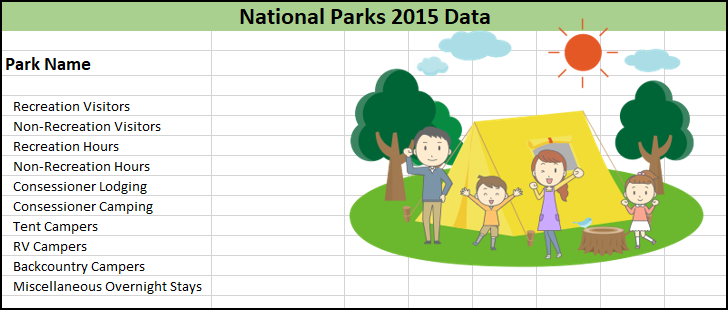
\includegraphics[width=\maxwidth{.95\linewidth}]{gfx/ch06_fig17}
	\caption{Sample setup}
	\label{06:fig17}
\end{figure}

\begin{enumerate}
	\item Make a copy of the \fmtWorksheetName{Park Data} sheet and rename it \fmtWorksheetName{Summary Park Data}. Change any text needed for the Summary sheet. Make sure both sheets are laid out exactly the same.
	\item Save the file as a template called \fmtWorkbookName{SC6 National Parks Template.xltx}. Make sure this gets saved to a USB drive and not the default folder on the hard drive. Close the template once it has been saved.
	\item Make a new file using the template and save it as \fmtWorkbookName{SC6 Five National Parks.xlsx}.
	\item Make four copies of the \fmtWorksheetName{Park Data} sheet. Rename the five Park Data sheets after the five parks listed in Table \ref{06:tab05}.
\end{enumerate}

\begin{table}[H]
	\rowcolors{1}{}{tablerow} % zebra striping background
	{\small
		%\fontsize{8}{10} \selectfont %Replace small for special font size
		\begin{longtable}{L{1.25in}L{0.70in}L{0.60in}L{0.70in}L{0.60in}} %Left-aligned, Max width: 4.25in
		\textbf{Name} & \textbf{Recreation Visitors} & \textbf{Non-recreation Visitors} & \textbf{Recreation Hours} & \textbf{Non-recreation Hours} \endhead
		\hline
		Acadia NP       & $ 2,811,184 $  & $ 47,100 $    & $ 14,452,151 $ & $ 47,100 $    \\
		Blue Ridge PKWY & $ 15,054,603 $ & $ 1,942,260 $ & $ 93,977,122 $ & $ 971,136 $   \\
		Crater Lake NP  & $ 614,712 $    & $ 49,600 $    & $ 4,033,484 $  & $ 24,800 $    \\
		Yellowstone NP  & $ 4,097,710 $  & $ 1,156,118 $ & $ 82,016,845 $ & $ 711,795 $   \\
		Yosemite NP     & $ 4,150,217 $  & $ 155,081 $   & $ 78,505,877 $ & $ 3,993,223 $ \\
		\rowcolor{captionwhite}
		\caption{National Park Data, Pt 1}
		\label{06:tab05}
		\end{longtable}
	}
\end{table}

\begin{table}[H]
	\rowcolors{1}{}{tablerow} % zebra striping background
	{\small
		%\fontsize{8}{10} \selectfont %Replace small for special font size
		\begin{longtable}{L{1.25in}L{0.60in}L{0.60in}L{0.60in}L{0.60in}} %Left-aligned, Max width: 4.25in
			\textbf{Name} & \textbf{Concessioner Lodging} & \textbf{Concessioner Camping} & \textbf{Tent Campers} & \textbf{RV Campers} \endhead
			\hline
			Acadia NP       & $ 0 $       & $ 0 $       & $ 135,000 $ & $ 32,094 $  \\
			Blue Ridge PKWY & $ 53,688 $  & $ 0 $       & $ 61,481 $  & $ 33,499 $  \\
			Crater Lake NP  & $ 34,629 $  & $ 55,596 $  & $ 7,548 $   & $ 0 $       \\
			Yellowstone NP  & $ 552,940 $ & $ 584,979 $ & $ 104,149 $ & $ 69,830 $  \\
			Yosemite NP     & $ 938,418 $ & $ 0 $       & $ 588,701 $ & $ 284,372 $ \\
			\rowcolor{captionwhite}
			\caption{National Park Data, Pt 2}
			\label{06:tab06}
		\end{longtable}
	}
\end{table}

\begin{table}[H]
	\rowcolors{1}{}{tablerow} % zebra striping background
	{\small
		%\fontsize{8}{10} \selectfont %Replace small for special font size
		\begin{longtable}{L{1.25in}L{0.60in}L{0.60in}} %Left-aligned, Max width: 4.25in
			\textbf{Name} & \textbf{Backcountry Campers} & \textbf{Misc Overnight Stays} \endhead
			\hline
			Acadia NP       & $ 1,233 $   & $ 8,343 $  \\
			Blue Ridge PKWY & $ 2,101 $   & $ 1,294 $  \\
			Crater Lake NP  & $ 3,253 $   & $ 0 $      \\
			Yellowstone NP  & $ 44,898 $  & $ 11,715 $ \\
			Yosemite NP     & $ 211,966 $ & $ 39,214 $ \\
			\rowcolor{captionwhite}
			\caption{National Park Data, Pt 3}
			\label{06:tab07}
		\end{longtable}
	}
\end{table}

\begin{enumerate}[resume]
	\item Enter the park data for each of the parks in each of the five sheets.
	\item In the \fmtWorksheetName{Summary Park Data} sheet, create formulas for all the fields that add up the five park sheets.
	\item Preview the entire workbook in Print Preview to ensure that it is printing professionally. Make any changes needed.
	\item Save the \fmtWorkbookName{SC6 Five National Parks} workbook.
	\item Submit both the \fmtWorkbookName{SC6 Five National Parks} and \fmtWorkbookName{SC6 National Parks Template} files as directed by the instructor.
\end{enumerate}

Note: The National Park 2015 Data is from: \url{https://irma.nps.gov/Stats/SSRSReports}.


